%!TEX root = ../main.tex

\section{Lightning Laplace}


\begin{frame}
\frametitle{Rational approximation in lightning solvers}
Consider the Laplace problem
\begin{eqnarray*}
	\nabla^2 u &=& 0 \quad\text{ in } \Omega,\\
	u &=& g \quad\text{ on } \partial\Omega_D,\\
	\uvec{n}\cdot\nabla u &=& h \quad\text{ on } \partial\Omega_N.
\end{eqnarray*}

$u$ will have singularities if $\Omega$ has corners or if $g$, $h$ are discontinuous along $\partial \Omega$ 
\begin{equation*}
f(z)\text{ analytic }\implies \nabla^2 \Re\left\{f(z)\right\} = 0
\end{equation*}

\bigskip
Rational functions are good for approximating functions with singularities
\begin{equation*}
f(z)\approx \sum_{j\in I} c_j r_j(z).
\end{equation*}

\end{frame}


\begin{frame}
\frametitle{Discretization: Least-squares fitting at the boundary}
We approximate $\left.u\right|_{\partial\Omega}$ by least-squares fitting at a discrete sample set of boundary points,
\begin{equation*}
A x \approx b,
\end{equation*}
\begin{itemize}
\item given $b\in\mathbb{R}^m$, the boundary data (Dirichlet / Neumann),
\item want $x\in\mathbb{R}^n$, containing the coefficients of $f(z)$,
\item  and $A\in\mathbb{R}^{m\times n}$, is the trace operator (samples $f(s_k), \{s_k\}\subset\partial\Omega$).
\end{itemize}

\begin{itemize}
\item More sampling points than fitting parameters $m\sim 3n$,
\item Non-unique solution, badly conditioned $\kappa(A)\sim 10^{16}$,
\item Dense linear algebra, $\texttt{x=A\textbackslash b}$.
\end{itemize}

\end{frame}



\begin{frame}
\frametitle{We choose our basis to be well conditioned and cheap to evaluate}
\begin{empheq}[box=\yellowbox]{align*}
f(z) \approx \sum_{k=0}^{N} a_k p_k (z) + \sum_{j=1}^{M} \frac{b_j}{z-z_j},
\end{empheq}
where $N=\mathcal{O}(\sqrt{M})$, and $p_k(z)\in \mathbb{P}_k$, $k=0,\ldots,N$ are \textbf{``Vandermonde with Arnoldi''} polynomials that obey a $(k+2)$-term recurrence
\begin{equation*}
H_{k+1,k} p_{k+1}(z) = z p_{k}(z) - \sum_{j=0}^{k} H_{j,k} p_j(z), \quad p_0(z)=1.
\end{equation*}
We can easily compute $f'(z)$ since
\begin{equation*}
H_{k+1,k} p'_{k+1}(z) = p_{k}(z) +z p'_{k}(z) - \sum_{j=1}^{k} H_{j,k} p'_j(z), \quad p'_0(z)=0.
\end{equation*}
\end{frame}




\begin{frame}
\frametitle{Our rational functions have fixed poles clustered near the corners}
The analysis guarantees root-exponential convergence $\mathcal{O}(\rho^{-\sqrt{M}})$ when
the poles $z_j$ corresponding to a corner $w$ are exponentially clustered
\begin{columns}
\begin{column}{0.4\linewidth}
\begin{figure}
	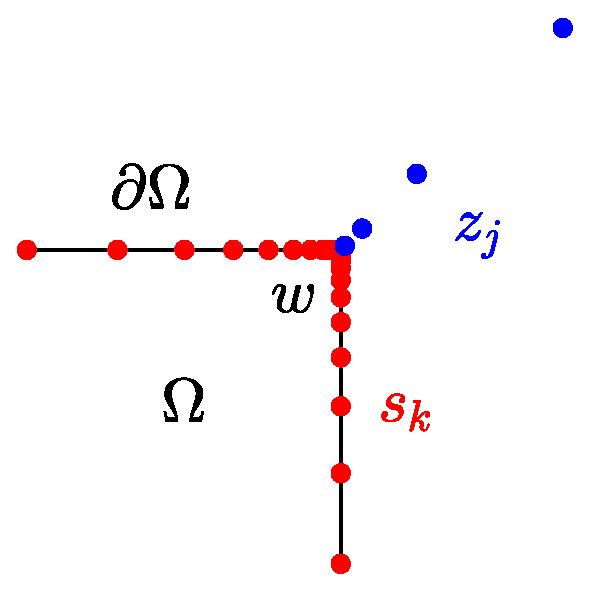
\includegraphics[height=0.9\linewidth]{Figures/cluster1}
\end{figure}
\end{column}
\begin{column}{0.6\linewidth}  
\begin{equation*}
|w-z_{j}| = L e^{-\sigma(\sqrt{M}-\sqrt{j})}, \quad j=1,\ldots,M.
\end{equation*}

\bigskip
The sample points $s_k$ on $\partial\Omega$ are chosen with the same clustering at the corner, but 3 times denser, i.e. $k=1,\dots,3M$ and $j\leftarrow k/3$ above.
\end{column}
\end{columns}
\vfill
\end{frame}

\begin{frame}
\frametitle{Now we want to deal with infinity}
\bigskip
Singularities at infinity can be resolved by exponentially spaced poles 
\begin{equation*}
\sigma\to -\sigma.
\end{equation*}
For unbounded domains, the sample points are also exponentially spaced.
\begin{figure}
	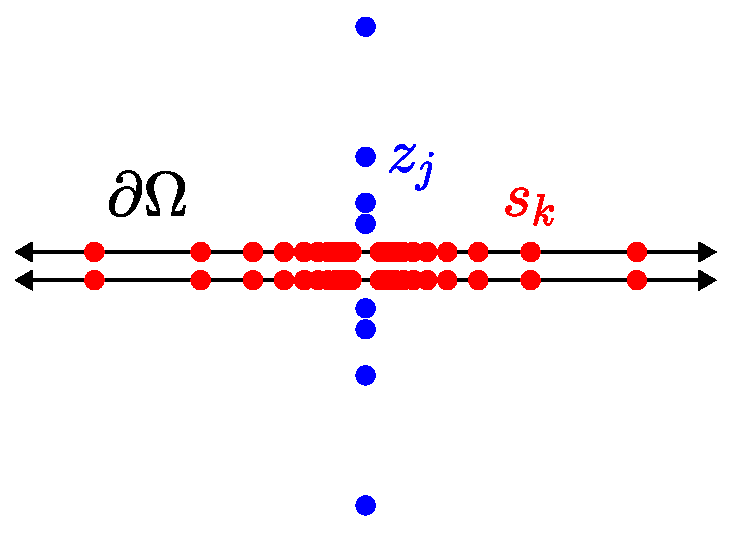
\includegraphics[height=0.45\linewidth]{Figures/cluster2}
\end{figure}
\end{frame}

\begin{frame}
\frametitle{Numerical example (u=1 at the top, u=0 at the bottom)}
\centering
\begin{figure}
	%\captionsetup{position=top}
	\subcaptionbox*{$-\infty\xleftarrow{\hspace*{0.4\linewidth}}x\xrightarrow{\hspace*{0.4\linewidth}}\infty$}{
		
\includegraphics[width=\linewidth]{Figures/lapchan_soln}}
	\vfill
	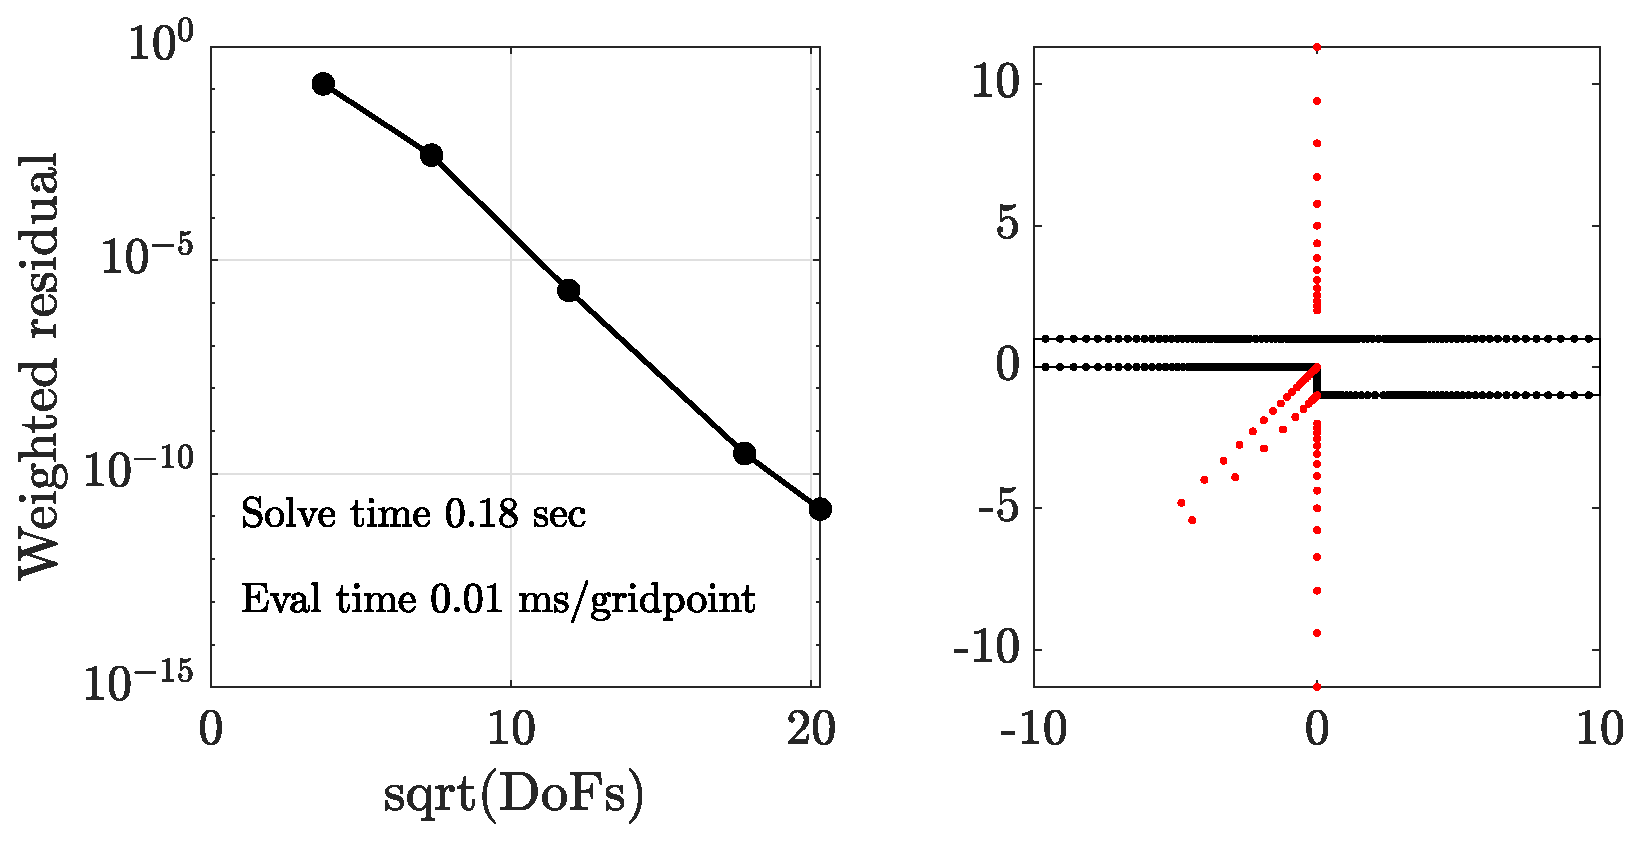
\includegraphics[height=0.3\linewidth]{Figures/lapchan_conv}
\end{figure}
\end{frame}


\begin{frame}
\frametitle{Multiply connected domains}
By the logarithmic conjugation theorem, if $u$ is harmonic on $\Omega$, then
\begin{equation*}
u = \Re\left\{f(z)\right\} + \sum_{j=1}^H \alpha_j \log\abs{z-h_j},
\end{equation*}
where $\{\alpha_j\}_{j=1}^H\subset\mathbb{R}$, and $h_j\in \mathbb{C}$ are points in each of the bounded components of the complement of $\Omega$ ($h_j$ is any point inside the $j$-th hole).
\end{frame}